\documentclass[10pt,a4paper,titlepage]{report}

\usepackage[utf8x]{inputenc}
\usepackage{float}
\usepackage{titlesec} 
\usepackage{listings}
\usepackage{url}
\usepackage{fullpage}
%


\usepackage{lmodern}
\usepackage[usenames,dvipsnames]{color}
\usepackage{geometry}
\geometry{scale=0.8, nohead}
\usepackage{t1enc}

\titleformat{\chapter}[hang]{\bf\huge}{\thechapter}{2pc}{} 

\author{Halloumi Fadi\\\texttt{halloumi@etud.insa-toulouse.fr}\\
Othacehe Mathieu\\\texttt{othacehe@etud.insa-toulouse.fr}\\
Volkmann Florian\\\texttt{volkmann@etud.insa-toulouse.fr}\\
Huynh Duc Ngoc\\\texttt{huynh@etud.insa-toulouse.fr}}

\title{Autonomous target-guided navigation in low obstacle enviroment}




%pour la cover page
\usepackage[pdftex]{graphicx}
\newcommand{\HRule}{\rule{\linewidth}{0.5mm}}
%pour afficher les listing
% theme listing 1
%\lstset{language=c,columns=flexible,caption=\lstname,
%numbers=left,stepnumber=5,numberfirstline=true,
%rangeprefix=//*,rangesuffix=*//,includerangemarker=false}
% theme listing 2
\definecolor{vert}{rgb}{0.2,0.6,0.4}
\lstset{language=c, breaklines=true, basicstyle=\ttfamily, keywordstyle=\color{blue}, commentstyle=\color{vert}, stringstyle=\color{red}, identifierstyle=\ttfamily}


%\fontfamily{lmss}
\begin{document}

\begin{titlepage}

\begin{center}


% Upper part of the page

\includegraphics[width=0.4\textwidth]{./imgs/logo_insa.png}\\[2cm]    

\textsc{\LARGE INSA Toulouse}\\[1.5cm]

\textsc{\Large Project Release Report }\\[0.5cm]


% Title
\HRule \\[0.4cm]
{ \huge  Autonomous Drone Guide}\\[0.4cm]

\HRule \\[1.5cm]

% Author and supervisor
\begin{minipage}{0.4\textwidth}
\begin{flushleft} \large
\emph{Engineers:}\\
Mathieu \textsc{Othacehe}\\
Florian \textsc{Volkmann}\\
Duc Ngoc \textsc{Huynh}\\
Fadi \textsc{Halloumi}\\
\end{flushleft}
\end{minipage}
\begin{minipage}{0.5\textwidth}
\begin{flushleft}
\large
\emph{Supervisors:} \\
Mr.Pierre-Emmanuel \textsc{Hladik}\\
Ms.Dinnah \textsc{McCarthy}\\
\emph{Mentor :} \\
Mr.Didier \textsc{Le Botlan}
\end{flushleft}
\end{minipage}

\vfill

% Bottom of the page
{\large Insa Toulouse 2013\copyright}

\end{center}

\end{titlepage}
 %coverpage
\maketitle %titlepage
\begin{abstract} %abstract page
Being fifth year students at INSA Toulouse, we saw that many visitors had difficulties to find the Electrical and Computer Engineering Department (DGEI) and they were late for the meeting. At the end of our study in Critical and Embedded System, we have an opportunity to work with a drone so we decided to make our project more useful. Our Pink team is working on developing a UAV that can go to DGEI wherever it was by searching a signal power of an Xbee emitter (or a GPS).
\end{abstract}

\tableofcontents %table of content
\clearpage


\chapter{Introduction}
Our team has been in charge to develop a guide to help people find their way at INSA. Our drone is able to converge to a target thanks to GPS coordinates. It is naturally able to fly in autonomy without human interactions.
// autre doc, pres plan

\chapter{General project presentation}
Our project is structure 
\chapter{Hardware considerations}
\section{Parrot 2.0}
The Parrot AR.Drone is a radio controlled flying quadrotor helicopter built by the French company Parrot. The drone is designed to be
controlled by any electronic device having wi-fi connection and sufficient ressource to run a control software. Only  android, iOS and windows have offically distributed control applications. In other hand, only Windows and Linux OS are supported as a development platform.
The choice of the department for this drone as a base for the project is due to the harmless character of this quadrotor.
Two versions of the Parrot AR.Drone exists. For our project only the new version(Ar.Drone 2.0) is supported.
\subsection{Ressources}
Many ressources could be found on this UAV and this what make it one of the best choices:
\begin{itemize}
\item \url{http://www.parrot.com/fr}
%\href{http://www.parrot.com/fr}{Parrot Official Website}
\item \url{http://ardrone.parrot.com/parrot-ar-drone/usa/}
%\href{http://ardrone.parrot.com/parrot-ar-drone/usa/}{Parrot Ardrone Commercial Website}
\item \url{http://projects.ardrone.org/}
%\href{http://projects.ardrone.org/}{Ardrone Project Website}
\item \url{http://devzone.parrot.com/}
%\href{http://devzone.parrot.com/}{Parrot Developpers Website}
\end{itemize}
\subsection{Specification}
Here a quick overview of the general specification of the drone:
\begin{itemize}
\item[-] Autonomy : Approximately 12 minutes, recharging time of 1h30.
\item[-] Maximum range : 50m average, 100m in a wide-open space with few Wi-Fi waves.
\item[-] Maximum altitude : 6m is the stability limitation, 50m the wi-fi limitation (which could be hacked with wi-fi booster to go up to 75m).
\item[-] Maximum additional supported weight : ~80g is the limit of stability, ~100g is the limit of motors propulsion.
\item[-] Maximum speed : 18 km/h.
\item[-] Maximum supported wind speed : 2km/h.

\end{itemize}

\subsection{Hardware}
The hardware reference is as follow:
\begin{itemize}
\item[*] AR.Drone 1.0 : carte Mykonos, processeur ARM926EJ-S rev 5 (v5l) Wi-Fi: AR6000 Memory: 128MB RAM
\item[*] AR.Drone 2.0 : Mykonos2 card, Processor OMAP 3640 1GHz 32 bit ARM Cortex A8 with a video DSP 800MHz TMS320DMC64x
\end{itemize}

\subsection{Software}
The board has an embedded Linux with these reference : \\
\begin{itemize}
\item[*] Linux myhost 2.6.27.47-parrot-01227-g93dde09 \#1 preempt Fri Jul 2 15:23:06 CEST 2010 armv5tejl GNU/Linux 
\item[*] Linux 2.6.32 kernel: Linux uclibc 2.6.32.9-g0d605ac \#1 preempt Fri Apr 6 12:01:59 CEST 2012 armv7l GNU/Linux 
\end{itemize}
This embedded linux contains these basic packages :
\begin{itemize}
\item[-] BusyBox
\item[-] Mtdutils
\item[-] zlib
\item[-] ethtool
\item[-] propcps
\item[-] udev
\item[-] dsp bridge 
\item[-] lcml dsp codec
\item[-] wireless tools
\item[-] exif
\item[-] iptables
\item[-] usbmodeswitch
\item[-] lsusb
\item[-] alsa lib
\item[-] barry
\item[-] busydroid
\item[-] webkit
\end{itemize}

We added multiple modules in order to be able to communicate with usb port:
\begin{itemize}
\item[-] cdc-acm 
\item[-] usbserial
\item[-] ftdi\_sio
\end{itemize}

you need to cross-compile these modules you can use the following steps :
\begin{enumerate}
\item Download an ARM Cross-compiler you can find one on the website of Mentor Graphics (successor of Code sourcery)\\ 
\url{http://www.mentor.com/embedded-software/sourcery-tools/sourcery-codebench/editions/lite-edition/arm-gnu-linux}
\item Install the cross-compiler :

\begin{lstlisting}
#: chmod +x arm-2012.03-57-arm-none-linux-gnueabi.bin
#: ./arm-2012.03-57-arm-none-linux-gnueabi.bin
\end{lstlisting}
\item Compile the module :
\begin{lstlisting}
#: /opt/CodeSourcery/Sourcery_CodeBench_Lite_for_ARM_GNU_Linux/bin/arm-none-linux-gnueabi-gcc -march=armv7-a toto.c -o toto.elf
\end{lstlisting}
\item Download and unzip Linux kernel: 
\begin{lstlisting}
#: wget --no-check certificate https://devzone.parrot.com/wiki/oss-ardrone2/Listing
#: tar zvxf linux.tar.gz
#: telnet 192.168.1.1
#: uname -a
#>  2.6.32.9-g0d605ac
\end{lstlisting}
Edit the Makefile in the root of Linux directory. The first fourth lines are VERSION (2), PATCHLvEL,  
SUBLEvEL (32) et EXTRAVERSION (.9).
Replace EXTRAVERSION = .9 by EXTRAVERSION = .9-g0d605ac to have the same version as the embedded linux.
\item Configurate the kernel :
\begin{lstlisting}
#: cd linux
#: cp kernel.config .config
#: make ARCH=arm menuconfig
\end{lstlisting}
Using the tool menuconfig , go to Device Drivers|USB Support . Tag the module as (M) in the corrosponding  ligne  USB Serial Converter 
support with the space key and then press enter to see the subdrivers. Tag (M) the ligne USB FTDI Single Port Serial Driver, finally, exit and save the file .config .
\item From the directory linux, compile the module :
\begin{lstlisting}
#: make ARCH=arm CROSS_COMPILE=/opt/CodeSourcery/Sourcery_CodeBench_Lite_for_ARM_GNU_Linux/bin/arm-none-linux-gnueabi- modules
\end{lstlisting}
\item Get  the compiled modules
The compiled modules are in the linux/drivers/usb/serial directory
\begin{lstlisting}
#: cp drivers/usb/serial/usbserial.ko ~
#: cp drivers/usb/serial/ftdi_sio.ko ~
\end{lstlisting}
\item check the installed modules
If you have doubt on the installed modules, Before to send them, you can check using the following command:
\begin{lstlisting}
#: /opt/CodeSourcery/Sourcery_CodeBench_Lite_for_ARM_GNU_Linux/bin/arm-none-linux-gnueabi-readelf -A ftdi_sio.ko
\end{lstlisting}
you should have probably have somthing like this output :
\begin{lstlisting}
File Attributes
  Tag_CPU_name: ``7-A''
  Tag_CPU_arch: v7
  Tag_CPU_arch_profile: Application
  Tag_ARM_ISA_use: Yes
  Tag_THUMB_ISA_use: Thumb-2
  Tag_ABI_PCS_wchar_t: 4
  Tag_ABI_FP_denormal: Needed
  Tag_ABI_FP_exceptions: Needed
  Tag_ABI_FP_number_model: IEEE 754
  Tag_ABI_align_needed: 8-byte
  Tag_ABI_align_preserved: 8-byte, except leaf SP
  Tag_ABI_enum_size: int
  Tag_ABI_optimization_goals: Aggressive Size
  Tag_CPU_unaligned_access: v6
  Tag_DIV_use: Not allowed
\end{lstlisting}
if the CPU\_name is 7-a, everthings is ok !
\item Loading the modules on the UAV
You can put the modules on the drone using ftp :
\begin{lstlisting}
#: cd ~
#: ftp 192.168.1.1
#: mput *.ko
#: exit
\end{lstlisting}
\item Mount the modules 
The modules are in the /data/video and the you can load them dynamically :
\begin{lstlisting}
#: telnet 192.168.1.1
#: cd /data/video
#: insmod usbserial ou insmod usbserial.ko
#: insmod ftdi_sio ou insmod ftdi_sio.ko
\end{lstlisting}
if needed you can use the two command lsmod to list the loaded modules and rmmod to remove a module.
\end{enumerate}

\subsection{Development}
\subsubsection{Install}
To install the SDK of the parrot please use the following script :
\begin{lstlisting}
#Create A project Directory
mkdir ~/Document/Projet_SEC && cd 
#Download the  SDK
wget --no-check certificate https://projects.ardrone.org/attachments/download/434/ARDrone_SDK_2_0.tar.gz
#Decompress the archive
tar -zxvf ARDrone_SDK_2_0.tar.gz
rm ARDrone_SDK_2_0.tar.gz
#Set the enviromment variables (Update the  Enviroment Variable and downloading the required packages)
source ARDrone_SDK_2_0/ARDroneLib/Soft/Build/check_dependencies.sh
#Test the configuration ( you will see ``Ok'' at the end if everthings is ok)
./ARDrone_SDK_2_0/ARDroneLib/Soft/Build/check_dependencies.sh
#Prepare the build for Linux (warning do NOT remove the spaces)
perl -p -i -e 's/USE_LINUX            = no/USE_LINUX            = yes/' ARDrone_SDK_2_0/ARDroneLib/Soft/Build/custom.makefile
#Compile the SDK
cd ARDrone_SDK_2_0/ARDroneLib/Soft/Build/ && make
#If New Curses is not installed you should do it
apt-get install libncurses5*
#Compile the examples
cd ../../../Examples/Linux/ && make
#Checking If examples Work (do not forget to connect to the drone wifi)
./Build/Release/ardrone_navigation
#Memorising SDK Path maybe you should put it in the .bashrc to avoid doing it every time
export ARDRONE_SDK=/home/<myuser>/Documents/Projet_SEC/ARDrone_SDK_2_0
\end{lstlisting}
\subsubsection{Connect to the drone:}
You could easiely use the the telnet commandline :
\begin{lstlisting}
telnet 192.168.1.1
\end{lstlisting}
\subsubsection{Change the configuration}
To change the default parameters used by the uav edit the file as follow :
\begin{lstlisting}
emacs -nw /data/config.ini
\end{lstlisting}

\subsubsection{Building An example}
The typic application structure is the following :\\
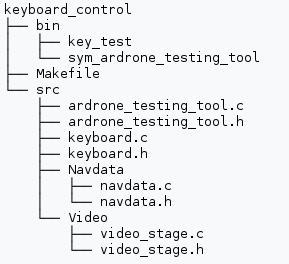
\includegraphics{imgs/structure_projet.png}

you can use the makefile sample :
\begin{lstlisting}
SDK_PATH:=$(ARDRONE_SDK)/ARDroneLib
PC_TARGET=yes
USE_LINUX=yes

ifdef MYKONOS
   include $(ARDRONE_CUSTOM_CONFIG)
   include $(ARDRONE_BUILD_CONFIG)
else
   include $(SDK_PATH)/Soft/Build/custom.makefile
   include $(SDK_PATH)/Soft/Build/config.makefile
endif

ifeq "$(RELEASE_BUILD)" "yes"
   ARDRONE_TARGET_DIR=$(shell pwd)/bin
else
   ARDRONE_TARGET_DIR=$(shell pwd)/bin
endif

TARGET=key_test

SRC_DIR:=$(shell pwd)/src

# Define application source files
GENERIC_BINARIES_SOURCE_DIR:=$(SRC_DIR)

GENERIC_BINARIES_COMMON_SOURCE_FILES+=			\
   Navdata/navdata.c    \
   Video/video_stage.c   \
   keyboard.c

GENERIC_INCLUDES+=					\
	$(SRC_DIR) \
	$(LIB_DIR) \
	$(SDK_PATH)/Soft/Common \
	$(SDK_PATH)/Soft/Lib

GENERIC_TARGET_BINARIES_PREFIX=

GENERIC_TARGET_BINARIES_DIR=$(ARDRONE_TARGET_DIR)

GENERIC_BINARIES_SOURCE_ENTRYPOINTS+=			\
   ardrone_testing_tool.c

GENERIC_INCLUDES:=$(addprefix -I,$(GENERIC_INCLUDES))

GENERIC_LIB_PATHS=-L$(GENERIC_TARGET_BINARIES_DIR)
GENERIC_LIBS=-lpc_ardrone -lgtk-x11-2.0 -lrt

SDK_FLAGS+="USE_APP=yes"
SDK_FLAGS+="APP_ID=key_test"

export GENERIC_CFLAGS
export GENERIC_LIBS
export GENERIC_LIB_PATHS
export GENERIC_INCLUDES
export GENERIC_BINARIES_SOURCE_DIR
export GENERIC_BINARIES_COMMON_SOURCE_FILES
export GENERIC_TARGET_BINARIES_PREFIX
export GENERIC_TARGET_BINARIES_DIR
export GENERIC_BINARIES_SOURCE_ENTRYPOINTS

# Bug fix ...
export GENERIC_LIBRARY_SOURCE_DIR=$(GENERIC_BINARIES_SOURCE_DIR)


.PHONY: $(TARGET) build_libs

all: build_libs $(TARGET)

$(TARGET):
	@$(MAKE) -C $(SDK_PATH)/VP_SDK/Build $(TMP_SDK_FLAGS) $(SDK_FLAGS) $(MAKECMDGOALS) USE_LINUX=yes
	mv $(ARDRONE_TARGET_DIR)/ardrone_testing_tool $(TARGET)
	mv $(TARGET) $(ARDRONE_TARGET_DIR)/

$(MAKECMDGOALS): build_libs
	@$(MAKE) -C $(SDK_PATH)/VP_SDK/Build $(TMP_SDK_FLAGS) $(SDK_FLAGS) $(MAKECMDGOALS) USE_LINUX=yes

build_libs:
	@$(MAKE) -C $(SDK_PATH)/Soft/Build $(TMP_SDK_FLAGS) $(SDK_FLAGS) $(MAKECMDGOALS) USE_LINUX=yes
\end{lstlisting}

You can test the application using these commands:
\begin{lstlisting}
#Open a new shell where you wich redirect the output of the example and check its id using **ps -p $**
# here in example the id is 5
./keyboar_control >> /dev/pts/5
\end{lstlisting}

\subsubsection{Building a video example}
To build or understand video you can use this example :
\begin{lstlisting}
cd $ARDRONE_SDK/Examples/Linux
wget --no-check-certificate https://projects.ardrone.org/attachments/download/466/ARDrone_SDK2_Video_Demo.zip
unzip ARDrone_SDK2_Video_Demo.zip
rm ARDrone_SDK2_Video_Demo.zip
make
\end{lstlisting}


\section{Ultrasonic Sensor}

\section{Bluetooth}

This part explains how to connect and read data from an android smartphone that sends information via bluetooth. ShareGPS, an application running on the phone is sending its GPS coordinate to the computer. The aim of the document is to give the process to get this coordinate.\\

First step: with the smartphone\\

\begin{itemize}
 \item Turn on the bluetooth and the GPS
 \item Launch ShareGPS and share coordinate via bluetooth
 \item Make the bluetooth visible by other devices
\end{itemize}

Second step: with the computer on Linux\\

\begin{itemize}
   \item  Turn on the bluetooth and open a terminal (you may need to be root)
   Scan devices with: ``hcitool scan''
   -> Write down the MAC address of the corresponding device
   \item Find the good channel which gives GPS coordinate with: ``sdptool records MAC\_ADDR''
   -> This command displays all channels and their functions
   -> Look for the one called ``ShareGPS'' and write down the corresponding channel
   \item Create the connection with: ``rfcomm bind X MAC\_ADDR CH''
    -> X: positive integer corresponding to the rfcomm you want to bind
    -> MAC\_ADDR: MAC address of the smartphone
    -> CH: channel of the ShareGPS application
\end{itemize}

You can now check that /dev/rfcommX exists. The last step is to read data.
To kill it use the command ``rfcomm release rfcommX'' or ``rfcomm release all''.\\

Third step: read data\\
\begin{itemize}
  \item Using PuTTY: connect via serial to /dev/rfcommX with a 9600 baudrate
  \item You can also use a self-made program
\end{itemize}

Source: \url{http://www.thinkwiki.org/wiki/How\_to\_setup\_Bluetooth}

\chapter{Software producted}
\section{Repository architecture}

The general architecture of our code repository is explained in this tree :\\

\begin{figure}[!h] 
\begin{center}
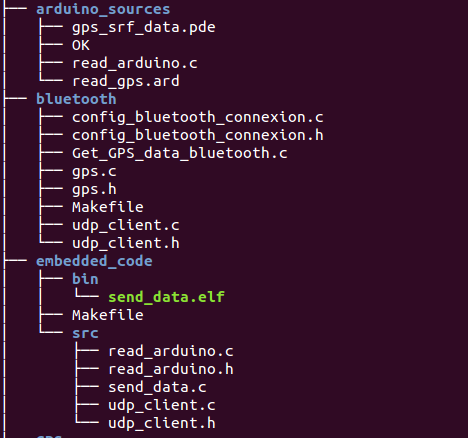
\includegraphics[width=10cm]{imgs/c1.png}
\caption{1st part of the repository} 
\label{img1} 
\end{center}
\end{figure} 

In arduino\_sources folder, all the code related to the arduino board can be found.
The software used to program the arduino is expecting .pde or .ard files.\\

In the following parts, we will provide more details for each files.\\

The bluetooth folder contains C sources et headers used on the target to catch informations sent by the smartphone.\\

The embedded code section includes all the programs we created to run on the UAV embedded linux.\\

\newpage

\begin{figure}[!h] 
\begin{center}
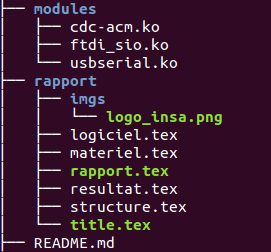
\includegraphics[width=7cm]{imgs/c2.png}
\caption{2nd part of the repository} 
\label{img1} 
\end{center}
\end{figure} 

All the compiled modules we added on the embedded linux can be found in the module folder.\\

The ``rapport'' directory contains the sources of the documentation you are reading !\\

Finally, the most important folder is the one named sdk\_apps. It contains one application named auto\_flight. Like most of the c projects, you can find a Makefile, a bin/ and a src/ folder. The Makefile is configurated to create the application binary and to move it to the bin/ folder. You can find additionnal informations about the Makefile in the appedices.\\

About the src/ folder :\\

The most important C file is named ardrone\_testing\_tool.c. This file is making the link between our application and the ARdrone library. Moreover, it is launching and joining all our threads.\\

The Auto/ folder contains code related to the auto\_control thread.\\

The Avoidance/ folder contains code related to the avoidance thread.\\

The Comm/ folder contains code related to the receive\_gps thread.\\

The Comm\_target/ folder contains code related to the gps\_target thread.\\

The Control/ folder contains an small library we wrote to handle UAV travelling.\\

The GPS/ folder contains algorithms used to manipulate GPS strings and make distance and angle calculation.

The Navdata/ folder contains the fonctions used to read and store navdata sent by the UAV.\\

The STMachine/ folder contains the fonctions generated by SCADE KCG compiler.\\

The Target/ folder contains code related to the target thread.\\

\begin{figure}[!h] 
\begin{center}
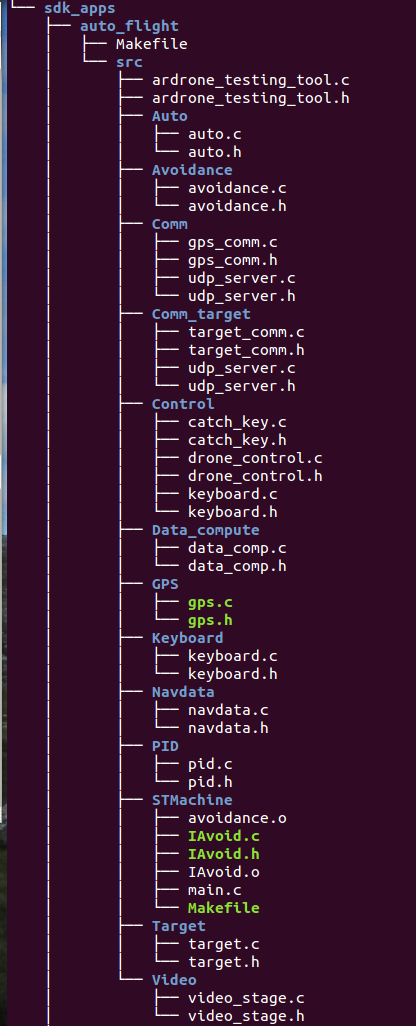
\includegraphics[width=8cm]{imgs/c3.png}
\caption{3rd part of the repository} 
\label{img1} 
\end{center}
\end{figure} 

\newpage{}

\begin{tabular}{|l|l|l|}
    \hline
    Thread name & Period & Description \tabularnewline
    \hline
    ardrone\_control & 2 & Library related thread \tabularnewline
    \hline
    navdata\_update & 20 & Library related thread \tabularnewline
    \hline
    auto\_control & 20 & Thread allowing manual command of the UAV \tabularnewline
    \hline
    receive\_gps & 50 & Thread used to received gps coordinated sent by the UAV  \tabularnewline
    \hline
    avoidance & 60    & Thread used to perform autonomous obstacle avoidance   \tabularnewline
    \hline
    gps\_target & 50 & Thread used to received gps coordinated sent by the target  \tabularnewline
    \hline
    gps\_target & 50 & Thread used to perform autonomous convergence to the target  \tabularnewline
    \hline

 \end{tabular}

This table summarizes all the thread launched in our application. In the following sections, we will detail the operations of each threads.

\section{The auto thread}

The auto thread is mainly based on the movement API we developped with the Brown team.\\

\subsection{Movement API}

This API is an overlay of the Parrot API, it allows more intuitive UAV control. It also provide movement quatification, which means you can quantify an order by speed, distance or duration. For example, you can emit orders like ``go forward on 300 cm''.

\subsubsection{Les mouvements élémentaires}

Les commandes de déplacement sont définis dans le fichier Control/drone\_control.c, elles ont toutes le même format :

The travelling commands are all defined in the file Control/drone\_control.c, they have the same format :\\

\begin{lstlisting}
C_RESULT ordre (void *arg)
\end{lstlisting}

The list of available travellings :\\

\begin{itemize}

\item turn\_left 
\item turn\_right
\item forward    
\item backward   
\item up         
\item down       
\item right      
\item left       
\item stop       

\end{itemize}

\subsection{Send an order}

The above order can be passed to both functions depending on whether you want to make a move that will be termed ``elementary'', or a longer trip by specifying the distance.

\subsubsection{Elementary move}

An elementary movement allows for a sudden displacement of around 10 cm. You must use the following function:

\begin{lstlisting}
C_RESULT small_move(ORDER* order)
\end{lstlisting}

Sample code :\\

\begin{lstlisting}
small_move(turn_right);
\end{lstlisting}

\subsubsection{Long move}

All orders to send move commands accept an argument of type void *. This argument must be cast to void * but available commands manage only the type arguments mov\_t which includes different arguments :\\

\begin{lstlisting}
typedef struct mov_t{
  int32_t power;     //engine power between 0 and 100 
  int32_t distance;  //distance in cm
  int32_t time;      //time in usec
}mov;
\end{lstlisting}

Before sending orders, it's important to fill correctly this structure. Unused fields must be initialized to -1. To send an order, this function must be used :\\

\begin{lstlisting}
C_RESULT send_order(ORDER* order, void *arg)
\end{lstlisting}

Sample code :\\

\begin{lstlisting}
/* 30% on 70 cm*/
mov mv = {30, 70, -1};
send_order(backward, &mv);
\end{lstlisting}

\subsection{Using of this API}

In the auto thread, we need to control the UAV with the keyboard of the station. This automatic control is really useful in case of problems occuring during the automatic control.\\

Basically, we are just running a scanf in an infinite loop. Depeding on the key pressed, we just have to call the wright function of the API.\\

\begin{lstlisting}
  while (1) {
    usleep(100000);
    scanf("%c", &c);
    printf("%c\n",c);
    switch(c){
    case 'f':
      small_move(forward);
      break;
    case 'b':
      small_move(backward);
      break;
    case 'u':
      small_move(up);
      break;
    case 'd':
      small_move(down);
      break;
    case 'o':
      //small_move(left);
      printf("Batt :%d\n",sauv_ndata.bat_level_current);
      break;
\end{lstlisting}

Very helpful functionalities are battery control, by pressing the ``o'' key, and recover from emergency m
ode by pressing ``x''. All the other command are pretty basic (``land'', ``go up'', ``go down'').\\

\subsection{Storing navdatas}

We also use this thread to store the navdata received. To achieve this goal, it is necessary to declare three functions, defined in the ARDrone library :\\

\begin{lstlisting}
/* Initialization local variables before event loop  */
inline C_RESULT auto_navdata_client_init( void* data )

/* Receving navdata during the event loop */
inline C_RESULT auto_navdata_client_process( const navdata_unpacked_t* const navdata )

/* Relinquish the local resources after the event loop exit */
inline C_RESULT auto_navdata_client_release( void )
\end{lstlisting}

We just keep the informations we have to use later, like battery level, control state, altitude or psi angle.

\begin{lstlisting}
  sauv_ndata.psi_current = nd->psi / 1000;
  sauv_ndata.bat_level_current = nd->vbat_flying_percentage;
  sauv_ndata.ctrl_state_current = nd->ctrl_state;
  sauv_ndata.tag_detected = nv->nb_detected;
  sauv_ndata.tag_tab = nv->camera_source;
  sauv_ndata.alt = nd->altitude / 1000.0;
\end{lstlisting}

We store all these informations in a global structure that will be accessed by the other threads.

\section{The avoidance thread}

This thread is mainly based on SCADE generated code. The statechart modeling the avoidance is printed below :\\

\begin{figure}[!h] 
\begin{center}

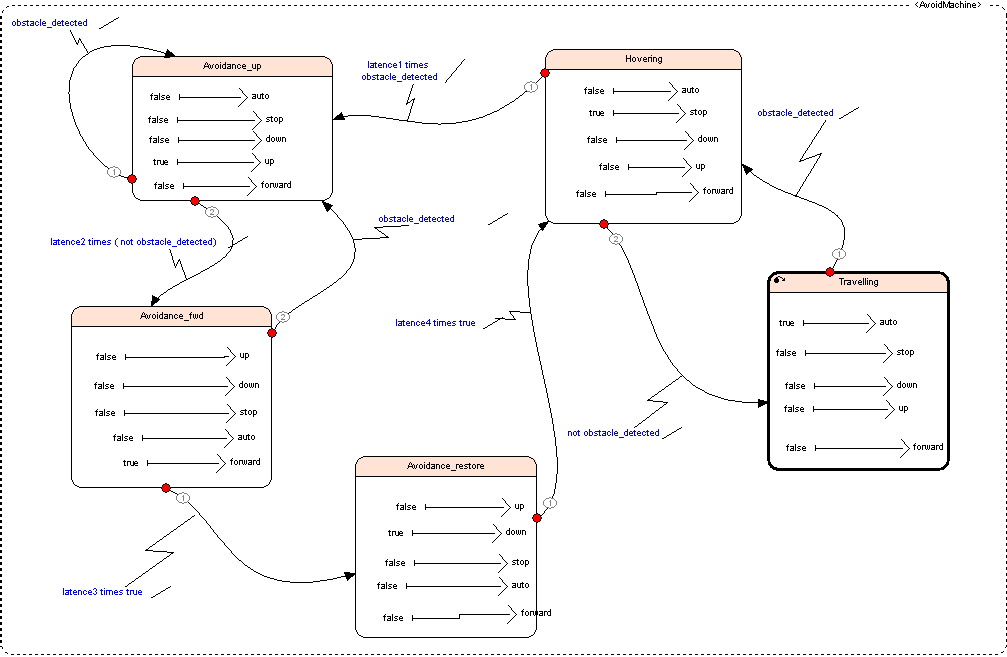
\includegraphics[width=19cm]{imgs/scade.png}
\caption{SCADE statechart} 
\label{img1} 
\end{center}
\end{figure} 

Then, the KCG compiler gave us some independent code, that we included in our project.

\begin{lstlisting}
switch (AvoidMachine_state_sel) {
    case SSM_st_Travelling_AvoidMachine :
      outC->AvoidMachine_reset_act = inC->obstacle_detected;
      break;
    case SSM_st_Hovering_AvoidMachine :
      if (br_1_guard_AvoidMachine_Hovering) {
        outC->AvoidMachine_reset_act = 1;
      }
      else {
        outC->AvoidMachine_reset_act = br_2_guard_AvoidMachine_Hovering;
      }
      outC->init = 0;
      break;
    case SSM_st_Avoidance_up_AvoidMachine :
      if (inC->obstacle_detected) {
        outC->AvoidMachine_reset_act = 1;
      }
      else {
        outC->AvoidMachine_reset_act = br_2_guard_AvoidMachine_Avoidance_up;
      }
      outC->init2 = 0;
      break;
\end{lstlisting}

The top-level function is defined in the file IAvoid.h.

\begin{lstlisting}
extern void IAvoid(inC_IAvoid *inC, outC_IAvoid *outC);
\end{lstlisting}

The inputs of this statechart are a boolean named ``obstacle\_detected'' (its value is 1 if there is an obstacle and 0 otherwise) and 4 integers describing latencies between transitions.\\

The outputs are 5 booleans : 4 orders (up, down, stop, forward) and a neutral order (if there is nothing to do).\\

Each call to the function represent a cycle. We have planned to execute a cycle each 10ms. The following code is illustrating the use of the auto-generated function :\\

\begin{lstlisting}
DEFINE_THREAD_ROUTINE(avoidance, data) {
  
  comm_datas datas;
  double dangerThreshold=100;
  int detection;
  double average_left;
  int ret;

  init_array_obstacle_pos2();

  IAvoid_reset(&output);
  input.obstacle_detected = 0;
  input.latence1 = 100;
  input.latence2 = 100;
  input.latence3 = 300;
  input.latence4 = 100;

 while (1) {
   usleep(10);
   if (auto_ready) {
     //get srf datas
     datas = get_comm_datas();

     ret = average_obstacle_pos2(&datas.srfr, &average_left);
     printf("Moyenne capteur(%d) : %f\n", ret, average_left);

     //check threshold
     if (average_left < dangerThreshold) {
       detection = 1;
     } else {
       detection = 0;
     } 
   
     input.obstacle_detected = detection;     
     IAvoid(&input,&output);
     command(output);
     usleep(10000);    
   }
 }
 
  return (THREAD_RET) 0;
}
\end{lstlisting}

And the command function is :\\

\begin{lstlisting}
void command(outC_IAvoid comm) {
  mov speed;

  if (comm.up) {
    speed.power = 8;
    send_fast_order(up,(void *)&speed);
  } else if (comm.down) {
    speed.power = 3;
    send_fast_order(down,(void *)&speed);
  } else if (comm.stop) {
    send_fast_order(stop,NULL);
  } else if (comm.auto1) {
    speed.power = 1;
    printf("avance\n");
    send_fast_order(forward,(void *)&speed);
  } else if (comm.forward) {
    speed.power = 1;
    printf("avance\n");
    send_fast_order(forward,(void *)&speed);
  }

}
\end{lstlisting}

\section{The receive\_gps \& gps\_target threads}

\section{The target thread}




\chapter{Final results}
\section{Autonomous flight}

At this point, we are able to launch a preplanned movements sequence. The movement library is quite sufficient to our needs.
The drone is stable even with additional weight. 
The following points  could be improved:

\begin{enumerate}
\item The movement library precision could be improved if the drone control model is developped.
\item The stability could be improved if the vertical speed is correctly boosted (it can be changed on the config.ini).
\item A PID could be used to add more fluency in the movements.
\item A study may be performed to repart more efficiently the addition weight.
\end{enumerate}

\section{Obstacle avoidance}
In the current state, the avoidance is performant. The drone is capable to avoid a fixed obstacle without any problem.
It can also avoid moving obstcales but it's still not reliable.
The following points could be improved:
\begin{enumerate}
\item The fluency of the avioidance could be improved with a PID (an implementation is already done still need to be tested).
\item The avoidance could bei extended to every obstacle using a second ultrasonic sensor, an arduino Mega because arduino Uno don't have sufficient hardware serial ports.
\item A more sophisticated automaton modelisation then the actual would make the avoidance highly performant.
\end{enumerate}

\section{Target convergence}

Currently, the target localisation and convergence is operational. The drone is able to localize the target, join it direction and stop within a defined range from it. The proximity convergence is not implemented yet but it will reuse programming blocks already developped like tag detection and small naviagtion movements defined in the movement library.The algorithm is pretty accurate and gives as an output the angle and the distance. Unfortunetly, the accumulated GPS errors make the distance precision very low but this fact is compensated by the proximity algorithm who uses image processing.

The following points could be improved :
\begin{enumerate}
\item The GPS errors could be very reduced using a kalmann filter. (please take note that the implementation of this filter is pretty complicated but the improvement will be tremendous).
\item A sophisticated image processing could be used to improve the calculated path.
\item A sophisticated scade automaton combined with a PID would improve the fluency of the movements.(A scade automaton already developped but not yet integrated neither tested)
\end{enumerate}




\chapter{Conclusion}
Conclusion

\end{document}

